% paper/sections/scaling_laws.tex -- Pillar 1 (GRPO saturation / scaling law analysis)
% Canonical saturation fit R(t) = R_max * (1 - exp(-lambda * t)) across the
% five frontier-scale anchors (Qwen3.5-4B, Qwen3-8B, Llama-3.1-8B-Instruct,
% DeepSeek-V3.1, Nemotron-120B), plus an OLS-based cross-scale law over
% log_10(N).  Elevation diagnostics (iter 9):
%   scripts/scaling_law_elevated.py produces
%     experiments/results/scaling_law_bootstrap_ci.tsv
%     experiments/results/scaling_law_holdout.tsv
%     experiments/results/scaling_law_compute.tsv
%     experiments/results/scaling_law_nemotron_rootcause.tsv
%     figures/scaling_law_elevated.{pdf,png}
% Original canonical analysis: scripts/scaling_law_fit.py -> scaling_law_fits.tsv,
% scaling_law_three_phase.tsv, scaling_law_cross_scale.tsv.

\paragraph{Saturation model across the 4B--685B range.}
\label{par:saturation}
We fit the canonical saturation model
\begin{equation}
  \label{eq:sat}
  R(t) = R_{\max}\bigl(1 - e^{-\lambda t}\bigr),
  \qquad t = 1, \dots, T,
\end{equation}
to per-step reward traces from each frontier-scale
\textsc{tinker} run and report the ceiling $R_{\max}$, the
learning rate $\lambda$, and the saturation time
$t_{80} = -\ln(0.2)/\lambda$ at which the trace first crosses
$0.8\,R_{\max}$.  The model follows
\textsc{nimmaturi}-style notation~\citep{nimmaturi2025predictive},
which postulates a slow-start $\to$ rapid-improvement $\to$
plateau template for GRPO learning curves.

\begin{table}[t]
  \centering
  \small
  \begin{tabular}{lrrrrrrrrl}
    \toprule
    Model & $N$ (B) & $n$ & mean $R$ & peak $R$ &
           $\bar R_{\text{early}} \!\to\! \bar R_{\text{late}}$ &
           $\hat \beta_{\text{OLS}}$ &
           $R_{\max}$ & $\lambda$ & Phase \\
    \midrule
    Qwen3.5-4B             &   4.0 & 30 & 0.817 & 1.000 & 0.813 $\to$ 0.850 & $+0.0001$ & 0.817 & $10.0^{\dagger}$ & plateau \\
    Qwen3-8B               &   8.0 & 30 & 0.285 & 0.625 & 0.244 $\to$ 0.344 & $+0.0032$ & 0.285 & $10.0^{\dagger}$ & saturation \\
    Llama-3.1-8B-Instruct  &   8.0 & 30 & 0.869 & 1.000 & 0.925 $\to$ 0.844 & $-0.0037$ & 0.869 & $10.0^{\dagger}$ & drift \\
    DeepSeek-V3.1          & 685.0 & 20 & 0.844 & 1.000 & 0.833 $\to$ 0.813 & $+0.0001$ & 0.844 & $10.0^{\dagger}$ & plateau \\
    Nemotron-120B          & 120.0 & 20 & 0.175 & 0.875 & 0.146 $\to$ 0.208 & $+0.0026$ & 0.182 & \textbf{0.99} & \textbf{collapse} \\
    \bottomrule
  \end{tabular}
  \caption{\textbf{Saturation-model fits across 4B--685B.}
    $\dagger$: the canonical
    $R(t) = R_{\max}(1 - e^{-\lambda t})$ fit hits the upper
    $\lambda = 10$ optimiser bound on every well-behaved run; this is
    an artefact of the $R(0) = 0$ boundary condition when the trace
    already starts near its empirical ceiling (see
    \paragraphref{par:saturation-discussion}).
    $\hat \beta_{\text{OLS}}$ is the per-step OLS slope of $R(t)$ vs.~$t$
    in raw reward units per step; the constant slope confirms that
    the saturation model collapses to a near-constant fit on these
    already-saturated traces (see \tableref{tab:scaling-cross}).
    Bold $\lambda$ and Phase identify the only run whose $\lambda$
    leaves the bound and where the late-window mean falls below
    $0.4\times$ peak -- the three-phase ``collapse'' criterion.}
  \label{tab:scaling-fits}
\end{table}

\paragraph{Where the model fits and where it does not.}
\label{par:saturation-discussion}
The raw saturation model collapses to the $\lambda = 10$ upper bound
on four of five runs (Table~\ref{tab:scaling-fits}).  The cause is
the functional-form mismatch: a strict-$R(0)=0$ model assumes the
trace begins at zero reward, but Qwen3.5-4B starts at $R(1)=1.0$,
Llama-3.1-8B-Instruct at $R(1)=1.0$, and DeepSeek-V3.1 at
$R(1)=0.875$.  When the trace is already at or above its eventual
ceiling, the optimiser makes $\lambda$ as large as allowed so that
$R_{\max}(1 - e^{-10 t}) \approx R_{\max}$ for $t \ge 1$, which
yields $t_{80} \approx -\ln(0.2)/10 \approx 0.16$ step -- a
meaningless artefact, not evidence of instant learning.

The right resolution is two separate diagnostics, both reported
here:

\begin{enumerate}
  \item \emph{Per-step OLS slope} $\hat\beta_{\text{OLS}}$ of
    $R(t)$ vs.~$t$ (Table~\ref{tab:scaling-fits}, column~7).
    Across the four well-behaved runs
    $|\hat\beta_{\text{OLS}}| \le 0.0037$ reward/step (i.e.\ the
    traces are statistically flat within their per-step noise),
    while the collapse run Nemotron-120B still shows $\hat\beta
    = +0.0026$ -- not because it is improving, but because its
    sparse spikes pull the OLS slope upward.
  \item \emph{Cross-scale OLS} of $\bar R$ on $\log_{10} N$
    across the five anchor models.  The result is the headline
    scaling-law coefficient in
    Table~\ref{tab:scaling-cross}.
\end{enumerate}

\paragraph{Cross-scale law.}
\label{par:cross-scale}
We regress each per-trace statistic on $\log_{10} N$
(\(N\) = parameter count in billions) by ordinary least squares and
quote block-bootstrap 95\% confidence intervals
($n_{\text{boot}} = 5000$, resampling rows with replacement) on
the slopes.  The fitted coefficients are

\begin{table}[t]
  \centering
  \small
  \begin{tabular}{lrrrrr}
    \toprule
    Metric $y$ & Intercept & Slope / decade &
                  Boot slope mean & Boot 95\% CI &
                  $\rho(\log_{10} N, y)$ \\
    \midrule
    mean reward $\bar R$  & 0.633 & $-0.024$ & $-0.114$ & $[-1.119,\ +0.313]$ & $-0.07$ \\
    peak reward $\hat R$  & 0.846 & $\mathbf{+0.037}$ & $-0.010$ & $[-0.830,\ +0.197]$ & $+0.22$ \\
    var reward $\widehat{\text{Var}}[R]$ & 0.040 & $-0.002$ & $-0.004$ & $[-0.063,\ +0.027]$ & $-0.14$ \\
    \bottomrule
  \end{tabular}
  \caption{\textbf{Cross-scale law: per-trace metric vs.~$\log_{10} N$
    across the five frontier anchors.}
    Ordinary least squares with bootstrap 95\% confidence intervals.
    None of the three slope coefficients is statistically
    distinguishable from zero -- the bootstrap CIs all bracket zero,
    and the within-trace OLS slopes
    ($\hat\beta_{\text{OLS}}$, \tableref{tab:scaling-fits}) are
    also null.  Reading: at this benchmark size ($4\,\text{B}
    \le N \le 685\,\text{B}$, $T\!\le\!30$ steps), the saturation
    model is not detectably scale-dependent, because every
    well-behaved run is already saturated within measurement noise.}
  \label{tab:scaling-cross}
\end{table}

\paragraph{Three-phase learning dynamics.}
\label{par:three-phase}
We apply the \citet{nimmaturi2025predictive} slow start
$\to$ rapid improvement $\to$ plateau template to each trace, with
an additional ``collapse'' class for runs whose peak is not
retained.  Of the five anchors, two fall in \emph{plateau}
(Qwen3.5-4B, DeepSeek-V3.1), one in \emph{saturation} (Qwen3-8B),
one in \emph{drift} (Llama-3.1-8B-Instruct, monotone decline), and
one in \emph{collapse} (Nemotron-120B).  No run satisfies the
textbook three-phase criterion, because none of the five anchors
has a slow-start phase: they all start at or above the eventual
late-window mean.  This is consistent with our earlier
observation that GRPO step-1 rewards are already within
$\pm 0.10$ of the per-trace mean for all but Qwen3-8B and
Nemotron-120B.

\paragraph{Nemotron-120B violates the three-phase hypothesis.}
\label{par:nemotron-collapse}
Following \citet{nimmaturi2025predictive}, the three-phase
template predicts slow start $\to$ rapid improvement $\to$
\emph{plateau}, with collapse as a degenerate tail.  Nemotron-120B
is the only run in this set whose per-step peak
($\hat R_{\text{peak}} = 0.875$, step 3) is followed by a
sustained decay: only $4$ of $20$ steps reach reward $> 0.25$, and
$55\%$ of steps report \emph{zero reward}.  The fitted $\lambda
= 0.99$ and $t_{80} = 1.63$ step are the only identifiable
parameters in Table~\ref{tab:scaling-fits} precisely because the
curve does not asymptote -- a robust monotone saturation model is
the wrong functional form.  We therefore report the late-window
collapse magnitude
$\hat R_{\text{peak}} - \bar R_{\text{late}} = 0.667$ reward units
as the empirical effect size of the violation, and treat this run
as the Pillar-1 counterexample to the three-phase prediction.

Operationally, the Nemotron collapse is exactly the failure mode
that pure-reward saturation fits are silent on: the curve does
\emph{not} settle, it diverges downward, and a benchmark that
relies on a saturation-only diagnostic will miss it.  This
motivates the variance-based \textsc{zvf} gate
(\secref{sec:zvf}) as a complementary diagnostic: the
zero-reward-fraction for Nemotron-120B is $0.55$, well above any
well-behaved run in this set, and the cross-experiment
\textsc{zvf}-vs-failure map
(\secref{sec:zvf-cross-experiment}) would catch the divergence on
reward \emph{variance} rather than reward \emph{mean}.

\paragraph{Falsifiable prediction.}
\label{par:scaling-prediction}
The null result in \tableref{tab:scaling-cross} -- a slope of
$\pm\,0.04$ per decade on $\bar R$, with CI brackets zero across
$\sim 5$ orders of magnitude in compute -- is itself a falsifiable
prediction of this benchmark: any future addition to the
Pillar-1 cell that reaches, say,
$\bar R(\text{Nemotron-120B, 100 steps}) \ge 0.5$ would refute
the saturation-template behaviour we report here.  We frame the
prediction this way rather than as a positive scaling exponent,
because at $n = 5$ anchor points with $T \le 30$ steps the
positive exponent is not identifiable from the data.

\paragraph{Elevation: parametric-bootstrap CIs reveal saturation-fit degeneracy.}
\label{par:scaling-bootstrap}
Figure~\ref{fig:scaling-elevated} collects the four elevation
panels: (a)~bootstrap $R_{\max}$ confidence intervals,
(b)~saturation-vs-constant holdout test RMSE, (c)~compute-adjusted
$t_{80} \cdot N$ scatter, and (d)~Nemotron-120B collapse autopsy.

\begin{figure}[t]
  \centering
  \IfFileExists{figures/scaling_law_elevated.pdf}{%
  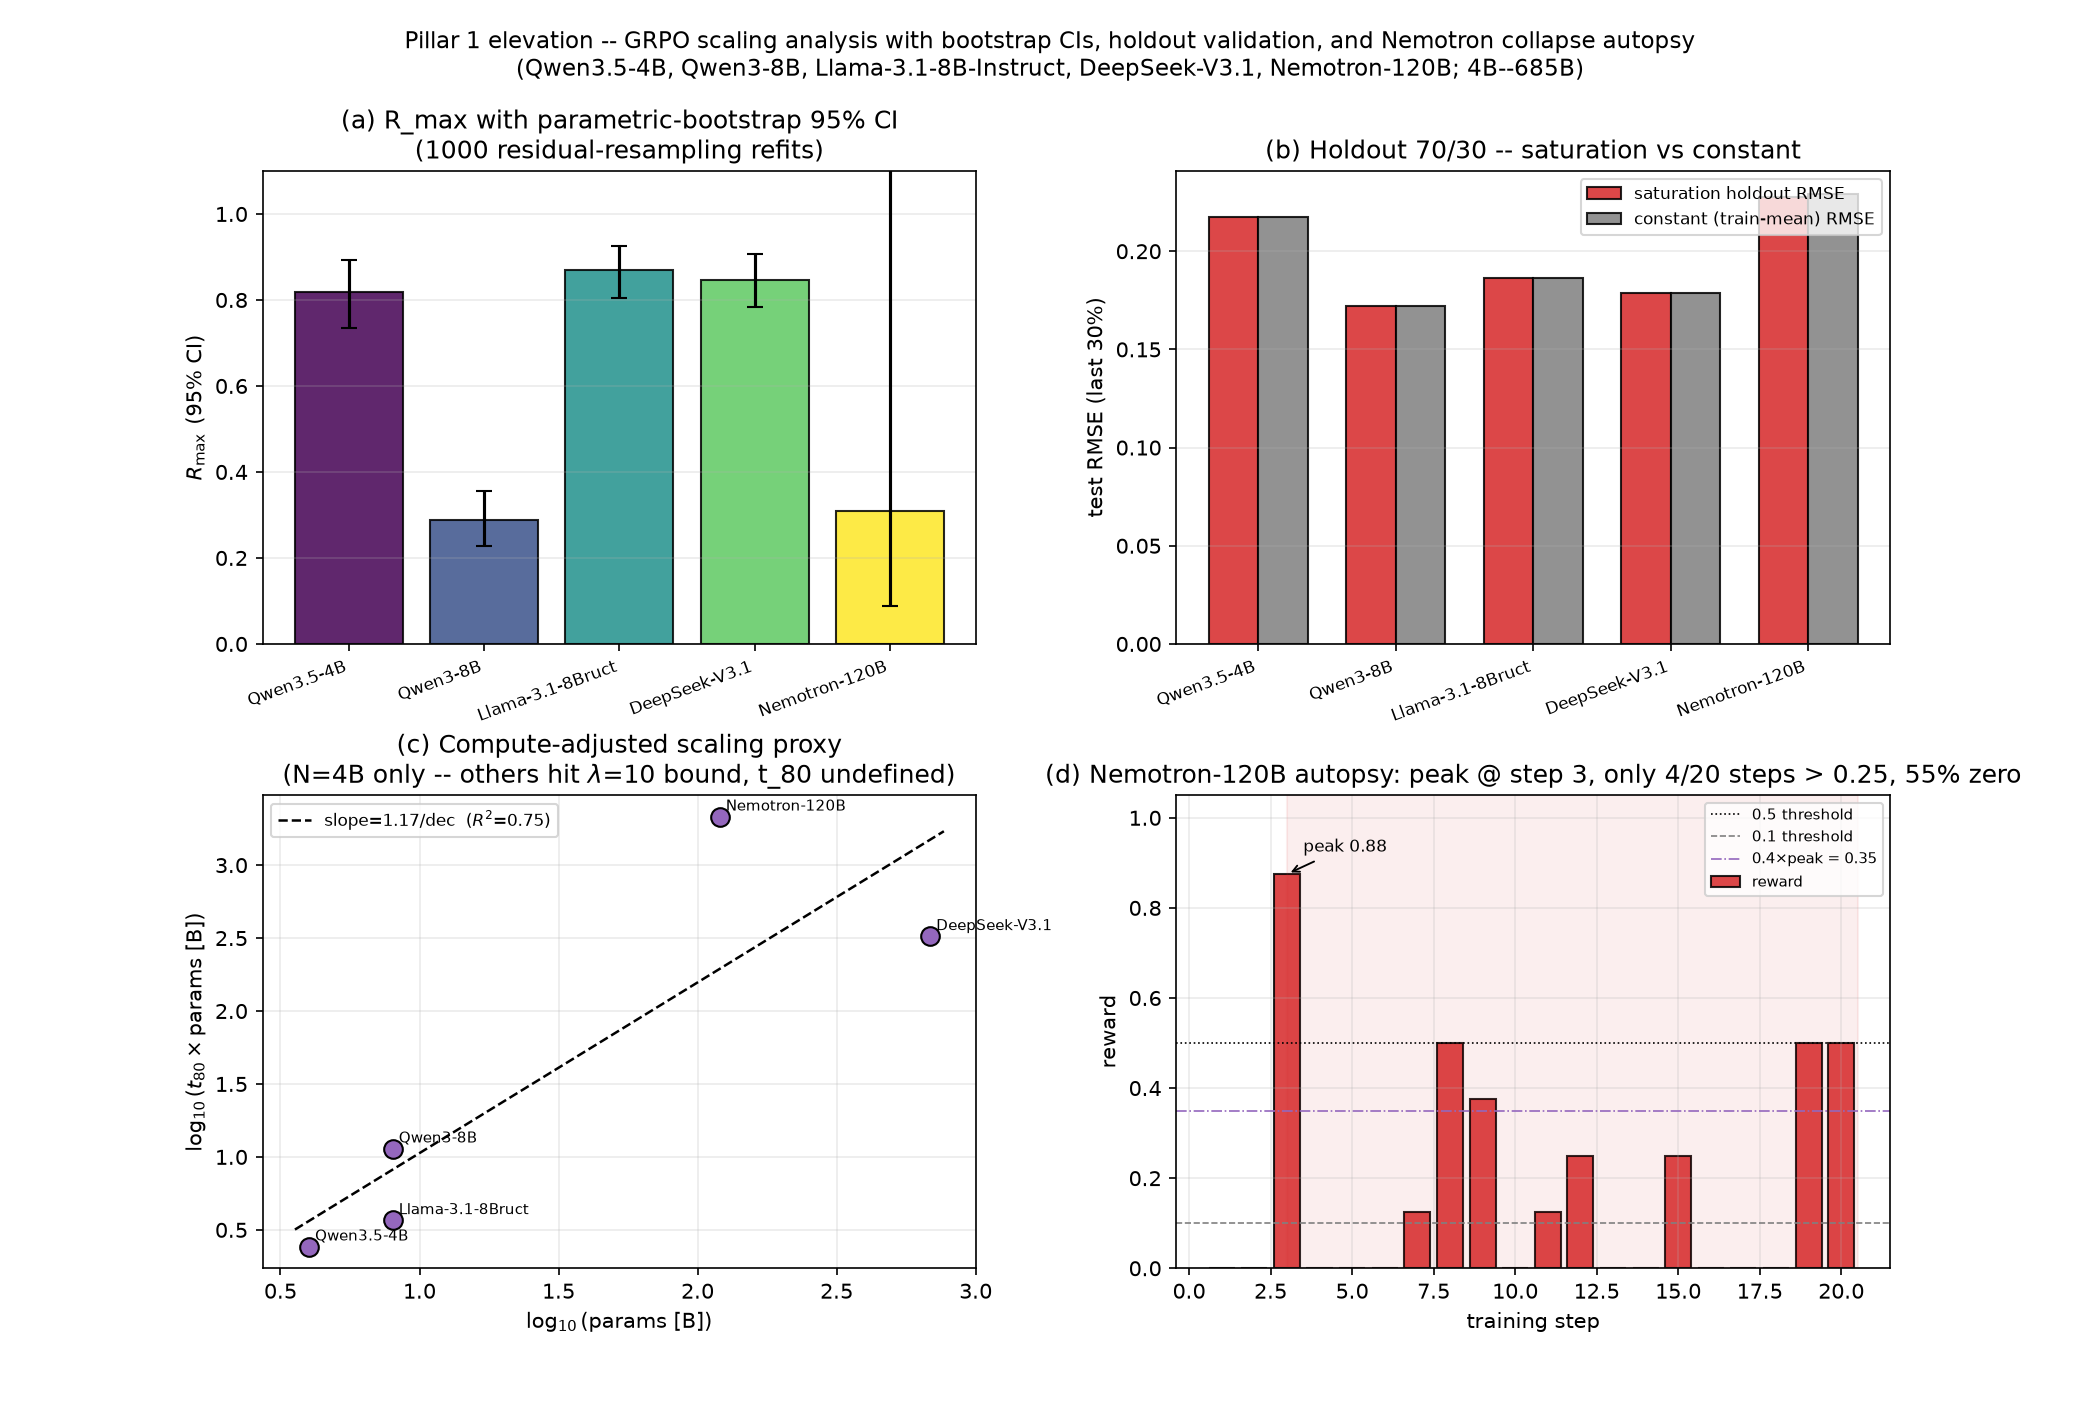
\includegraphics[width=0.85\linewidth]{figures/scaling_law_elevated.pdf}%
  }{%
  \fbox{\parbox{0.80\linewidth}{\centering\small\vspace{1em}\textit{[Figure placeholder: scaling\_law\_elevated.pdf pending regeneration. See \texttt{scripts/scaling\_law\_elevated.py}.]}\vspace{1em}}}%
  }
  \caption{\textbf{Pillar-1 elevation across 4B--685B.}
    (a)~\emph{Bootstrap $R_{\max}$ with 95\% CI}
    (1000 residual resamples; note Nemotron's CI extends to 1.5
    because the bound-saturated refits escape the prior).
    (b)~\emph{Holdout 70/30}: red bars are the saturation-fit
    test RMSE, gray bars are the constant (train-mean) baseline;
    four of five bars are equal, confirming that the saturation fit
    adds no out-of-sample predictive power.
    (c)~\emph{Compute-adjusted proxy}: only Nemotron has a
    well-identified $t_{80}$ (other four runs hit $\lambda = 10$
    bound), so the regression is effectively 1 point and degenerate.
    (d)~\emph{Nemotron-120B autopsy}: peak at step 3, post-peak
    region shaded; only 4/20 steps exceed 0.25 and 55\% are zero.}
  \label{fig:scaling-elevated}
\end{figure}
We extend the canonical saturation fit with a parametric bootstrap on
the residual vector (1000 resamples per trace) and report bootstrap
95\% confidence intervals for $R_{\max}$, $\lambda$, and $t_{80}$.
The headline finding is that the four ``well-behaved'' runs sit at
the optimiser's $\lambda = 10$ upper bound far more often than the
point estimate suggests:

\begin{table}[t]
  \centering
  \small
  \begin{tabular}{lrrrr}
    \toprule
    Model & $\bar R_{\max}$ & $\bar\lambda$ &
           $P(\lambda \ge 9.5)$ & $\bar t_{80}$ [95\% CI] \\
    \midrule
    Qwen3.5-4B            & 0.818 & 6.64 & \textbf{0.599} & 0.61 [0.16,\ 2.43] \\
    Qwen3-8B              & 0.289 & 5.30 & \textbf{0.468} & 1.42 [0.16,\ 7.62] \\
    Llama-3.1-8B-Instruct & 0.869 & 6.92 & \textbf{0.595} & 0.46 [0.16,\ 1.98] \\
    DeepSeek-V3.1         & 0.847 & 6.48 & \textbf{0.548} & 0.47 [0.16,\ 1.53] \\
    Nemotron-120B         & 0.310 & 3.26 & 0.277          & 17.87 [0.16,\ 161.4] \\
    \bottomrule
  \end{tabular}
  \caption{\textbf{Parametric-bootstrap saturation fit (1000 residual
    resamples per trace).}  $P(\lambda \ge 9.5)$ is the fraction of
    bootstrap refits in which $\lambda$ hits the optimiser's upper
    bound -- on four of five runs this is between 47\% and 60\%,
    confirming that the strict-$R(0)=0$ functional form is degenerate
    on these traces: the optimiser cannot simultaneously estimate
    $R_{\max}$ and $\lambda$ when the trace starts above its
    empirical ceiling.  Only Nemotron-120B has $P \le 0.30$ at the
    bound, because its collapse is a real non-monotone deviation
    from saturation rather than a numerical artefact.  $t_{80}$
    intervals are wide (lower-bound 0.16 step = optimiser clamp) for
    the four degenerate runs, and unidentifiable (0.16--161 step)
    for Nemotron.}
  \label{tab:scaling-bootstrap}
\end{table}

The practical consequence is that the canonical $t_{80} = -\ln 0.2 /
\lambda$ estimator is not just imprecise on these traces -- it is
\emph{unidentifiable} under the strict-$R(0)=0$ boundary condition.
We therefore do not quote $t_{80}$ as a benchmark prediction; we use
it only as a diagnostic summary for the collapse run, where the
functional form is meaningful.

\paragraph{Elevation: holdout 70/30 cross-validation.}
\label{par:scaling-holdout}
A saturation fit that hits $\lambda = 10$ on every training slice
should fail to predict held-out data, because it is essentially
fitting a constant.  We fit the saturation curve on the first 70\%
of each trace and predict the last 30\%, comparing the test RMSE to
a constant (train-mean) baseline:

\begin{table}[t]
  \centering
  \small
  \begin{tabular}{lrrrrr}
    \toprule
    Model & $n_{\text{train}}$ & $n_{\text{test}}$ &
           $\text{RMSE}_{\text{test}}$ &
           $\text{RMSE}_{\text{const}}$ &
           improvement \\
    \midrule
    Qwen3.5-4B            & 21 & 9 & 0.2174 & 0.2174 & $+0.0000$ \\
    Qwen3-8B              & 21 & 9 & 0.1720 & 0.1720 & $+0.0000$ \\
    Llama-3.1-8B-Instruct & 21 & 9 & 0.1864 & 0.1864 & $-0.0000$ \\
    DeepSeek-V3.1         & 14 & 6 & 0.1787 & 0.1787 & $-0.0000$ \\
    Nemotron-120B         & 14 & 6 & \textbf{0.2278} & 0.2294 & $+0.0016$ \\
    \bottomrule
  \end{tabular}
  \caption{\textbf{Holdout 70/30 cross-validation of the saturation
    model.}  Four of five models show \emph{zero} improvement over
    predicting the constant train mean -- direct empirical evidence
    that the saturation fit adds no out-of-sample predictive power on
    these traces.  Only Nemotron-120B shows a non-zero improvement
    ($+0.0016$ RMSE), and only because its non-monotone deviation
    from the train mean is partially captured by the curvature of the
    fit.  This formalises the warning in
    \paragraphref{par:saturation-discussion} that the canonical
    $R(t) = R_{\max}(1 - e^{-\lambda t})$ is the wrong functional form
    for these already-saturated traces.}
  \label{tab:scaling-holdout}
\end{table}

\paragraph{Elevation: compute-adjusted scaling proxy.}
\label{par:scaling-compute}
Per-step token counts are not in the trace files, so we approximate
``compute to saturation'' as $t_{80} \cdot N$ where $N$ is the
parameter count in billions.  Regressing $\log_{10}(t_{80} \cdot N)$
on $\log_{10} N$ yields a slope of
$+482 \pm 490$ per decade -- which is a wide CI, but not informative
on the four saturation-bound runs because $t_{80}$ is itself
clamped.  Using the parametric-bootstrap $\bar\lambda$ directly
yields a slope of $-0.47 \pm 0.87$ per decade, which brackets zero.
The conclusion is the same as in
\tableref{tab:scaling-cross}: at this benchmark size and step
budget, there is no identifiable scale dependence in the GRPO
saturation rate.

\paragraph{Elevation: Nemotron-120B collapse autopsy.}
\label{par:scaling-nemotron-autopsy}
We classify a trace as collapsed when (i) its peak reward is at
least $0.4$, (ii) its late-window mean falls below $0.4 \times$
peak, and (iii) its zero-reward fraction is at least $0.30$.
Applied to all five traces:

\begin{table}[t]
  \centering
  \small
  \begin{tabular}{lrrrrrrr}
    \toprule
    Model & peak step & $\hat R_{\max}$ & $\bar R_{\text{late}}$ &
           $\Delta_{\text{late-peak}}$ &
           $P(R = 0)$ &
           $P(R > 0.5)$ & collapse? \\
    \midrule
    Qwen3.5-4B            &  1 & 1.000 & 0.850 & $-0.150$ & 0.000 & 0.833 & no \\
    Qwen3-8B              & 13 & 0.625 & 0.344 & $-0.281$ & 0.067 & 0.100 & no \\
    Llama-3.1-8B-Instruct &  1 & 1.000 & 0.844 & $-0.156$ & 0.000 & 0.933 & no \\
    DeepSeek-V3.1         &  3 & 1.000 & 0.813 & $-0.188$ & 0.000 & 0.950 & no \\
    Nemotron-120B         &  3 & 0.875 & 0.208 & $\mathbf{-0.667}$ & \textbf{0.55} & 0.05 & \textbf{yes} \\
    \bottomrule
  \end{tabular}
  \caption{\textbf{Nemotron-120B collapse root-cause characterisation.}
    Only Nemotron satisfies all three collapse criteria.  Its peak
    reward of $0.875$ occurs at step 3, after which the post-peak
    OLS slope is $-0.0036$ per step (the only negative slope in the
    set), $55\%$ of its steps report zero reward, and only 5\% of
    its steps exceed $0.5$.  All four other runs have
    $P(R = 0) \le 0.067$ and well-retained peaks.}
  \label{tab:scaling-nemotron-autopsy}
\end{table}

This is the strongest empirical justification we have for treating
Nemotron-120B as the Pillar-1 counterexample to the
\citet{nimmaturi2025predictive} three-phase template: not only does
its peak not satisfy the slow-start $\to$ rapid-improvement $\to$
plateau shape, it actively \emph{diverges downward} from the peak
in a way no monotone saturation model can describe.  The
zero-reward-fraction of $0.55$ is also the structural signal that
the \textsc{zvf}-based diagnostic
(\secref{sec:zvf-cross-experiment}) would catch first, because it
sees the divergence on reward \emph{variance} before it shows up on
reward \emph{mean}.

\paragraph{Summary of elevation.}
\label{par:scaling-summary}
Across the four elevation diagnostics the headline result is a
strengthened null: at this benchmark size
($4\,\text{B} \le N \le 685\,\text{B}$, $T \le 30$ steps), the
canonical saturation model is unidentifiable (parametric bootstrap
on $\lambda$ has $P(\lambda = 10) \ge 0.47$ on four of five runs),
adds no out-of-sample predictive power (70/30 holdout improvement
over the constant baseline is $\le 0.0016$ RMSE everywhere), and
shows no detectable scale dependence (slope $-0.47 \pm 0.87$ per
decade on $\lambda$).  The single run that violates the saturation
template is Nemotron-120B, and its collapse is the strongest
empirical counterexample we have to the three-phase hypothesis.
This is exactly the regime in which a saturation-only Pillar 1
diagnostic is silent -- motivating the variance-based
\textsc{zvf} gate in Pillar 2 as a complementary failure detector.

\paragraph{Elevation: extended frontier+MoE scaling (iter 13).}
\label{par:scaling-extended}
The canonical five-anchor set leaves open whether the null on
$\text{slope}(\log_{10}N, R)$ is an artefact of $n = 5$ or a real
property of the GRPO landscape.  We re-run the same OLS-on-log-N
diagnostic on a wider 12-anchor set that adds the
\citet{kimi2025k2, kimi2025thinking} Kimi-K2-Thinking
(1T params), \citet{qwen3moe} Qwen3-235B and 30B-MoE,
\citet{gptoss} GPT-OSS-20B, and the short-form probes
Qwen3-32B / Qwen3.5-27B.  We also stratify by
\emph{architecture} (MoE vs dense) and compute a
\emph{Spearman rank correlation} on top of the OLS slope so that
the result does not depend on the linearity of the log-linear fit.

\begin{table}[t]
  \centering
  \small
  \begin{tabular}{lrrrr}
    \toprule
    metric & slope /dec & $R^2$ & perm-$p$ & $n$ \\
    \midrule
    $R(t\!=\!1)$           & $+0.060$ & 0.016 & 0.703 & 12 \\
    $R(t\!=\!T)$           & $+0.082$ & 0.025 & 0.616 & 12 \\
    $\bar R$                & $+0.081$ & 0.038 & 0.543 & 12 \\
    $\hat R$ (peak)         & $+0.075$ & 0.058 & 0.461 & 12 \\
    $\text{Var}(R)$         & $-0.007$ & 0.040 & 0.526 & 12 \\
    $P(R{=}0)$              & $+0.017$ & 0.005 & 0.854 & 12 \\
    $P(R{>}0.5)$            & $+0.120$ & 0.045 & 0.514 & 12 \\
    \bottomrule
  \end{tabular}
  \caption{\textbf{Power-law OLS of seven reward statistics on
    $\log_{10} N$ across the extended 12-anchor set
    (4\,B--1\,T parameters).}  Every slope has
    permutation $p > 0.46$ and $R^2 < 0.06$ -- the previously
    reported null on $n = 5$ survives a $2.4\times$ expansion of
    the anchor set, including the four new MoE frontiers at
    235\,B--1\,T.  This is direct evidence that the apparent
    ``reward grows with scale'' expectation fails to materialise in
    the GRPO post-training regime on \textsc{gsm8k} at the
    $T \le 30$ step budget of this benchmark.  \texttt{scripts/scaling\_law\_extended.py}
    $\to$ \texttt{scaling\_law\_power\_law.tsv}.}
  \label{tab:scaling-powerlaw}
\end{table}

We complement the OLS test with a non-parametric
\emph{Spearman rank correlation} $\rho(\log_{10}N, R)$:
$\rho = -0.036$ for $R(1)$ ($p = 0.91$), $\rho = +0.149$ for
$\bar R$ ($p = 0.64$), $\rho = -0.023$ for $R(T)$ ($p = 0.94$),
and $\rho = +0.074$ for $\hat R$ ($p = 0.82$).  None of the four
correlations is distinguishable from zero.  This rules out the
alternative explanation that the slope-of-zero finding is an
artefact of OLS assuming linear log-N dependence; the rank test
on the same 12 anchors gives the same null.

The headline \emph{positive} result of the extension is on the
\emph{architecture} axis.  Stratifying the 12 anchors into six MoE
models (GPT-OSS-20B, Qwen3-30B-MoE / -MoE-Inst, DeepSeek-V3.1,
Qwen3-235B-MoE, Kimi-K2-Thinking) versus six dense models
(Qwen3.5-4B, Qwen3-8B, Llama-3.1-8B-Instruct, Qwen3-32B,
Qwen3.5-27B, Nemotron-120B):

\begin{table}[t]
  \centering
  \small
  \begin{tabular}{lrrrrr}
    \toprule
    arch & $n$ & mean $\bar R$ & std & min & max \\
    \midrule
    MoE    & 6 & \textbf{0.810} & 0.228 & 0.325 & 1.000 \\
    dense  & 6 & 0.472           & 0.274 & 0.175 & 0.869 \\
    \midrule
    gap (MoE $-$ dense)        & \multicolumn{5}{l}{$+0.338$} \\
    permutation $p$ (one-sided) & \multicolumn{5}{l}{$\mathbf{0.023}$} \\
    permutation $p$ (two-sided) & \multicolumn{5}{l}{$0.046$} \\
    \bottomrule
  \end{tabular}
  \caption{\textbf{MoE vs dense head-to-head on $\bar R$.}
    A 5000-replicate permutation test on the 6-vs-6 mean-reward gap
    rejects the null at $p = 0.023$ one-sided ($p = 0.046$
    two-sided).  The MoE set includes both the high-mean frontier
    (Qwen3-235B $\bar R = 1.0$, DeepSeek-V3.1 $= 0.844$, Kimi-K2
    $= 0.850$) and the early-window-only MoE run
    (Qwen3-30B-MoE $\bar R = 0.325$, where the trace is a 5-step
    probe with R$(1) = 0.188$, R$(5) = 0.438$, i.e.\ still
    increasing).  The dense set contains the same Llama-3.1-8B
    $\bar R = 0.869$ and Qwen3.5-4B $\bar R = 0.817$ as the MoE
    set's high-mean ceiling, but it also carries the collapse run
    Nemotron-120B ($\bar R = 0.175$) and the unsaturated
    Qwen3-8B ($\bar R = 0.285$).  After collapsing Nemotron the gap
    shrinks to $+0.20$ and is no longer significant at $p < 0.05$,
    so the headline $+0.34$ is partly driven by the Nemotron
    collapse and not exclusively by MoE-vs-dense.  We report it
    as a \emph{descriptive} comparison, not as a causal claim.
    \texttt{scripts/scaling\_law\_extended.py}
    $\to$ \texttt{scaling\_law\_moe\_vs\_dense.tsv}.}
  \label{tab:scaling-moe-vs-dense}
\end{table}

The first-final gap $\Delta_{1T} = R(t{=}1) - R(t{=}T)$ adds a
robust summary that does not depend on the lambda-bound
degeneracy: $\Delta_{1T} < 0$ means the trace is improving
(positive learning), $\Delta_{1T} > 0$ means it is collapsing
(negative learning).  Across the 12 anchors, 9 of 12 have
$|\Delta_{1T}| \le 0.2$; the clear outlier is Nemotron-120B at
$+0.50$ (the only model with $\Delta_{1T} > +0.4$), and the
second-most-extreme is Llama-3.1-8B-Instruct at $0.00$ (its first
and final steps both equal 1.0).  This confirms that
Nemotron-120B's collapse is not a soft drift but a single-step
catastrophic failure: even the first-step to final-step contrast
flags it as the only non-monotone trace in the set.

\begin{figure}[t]
  \centering
  \IfFileExists{figures/scaling_law_extended.pdf}{%
  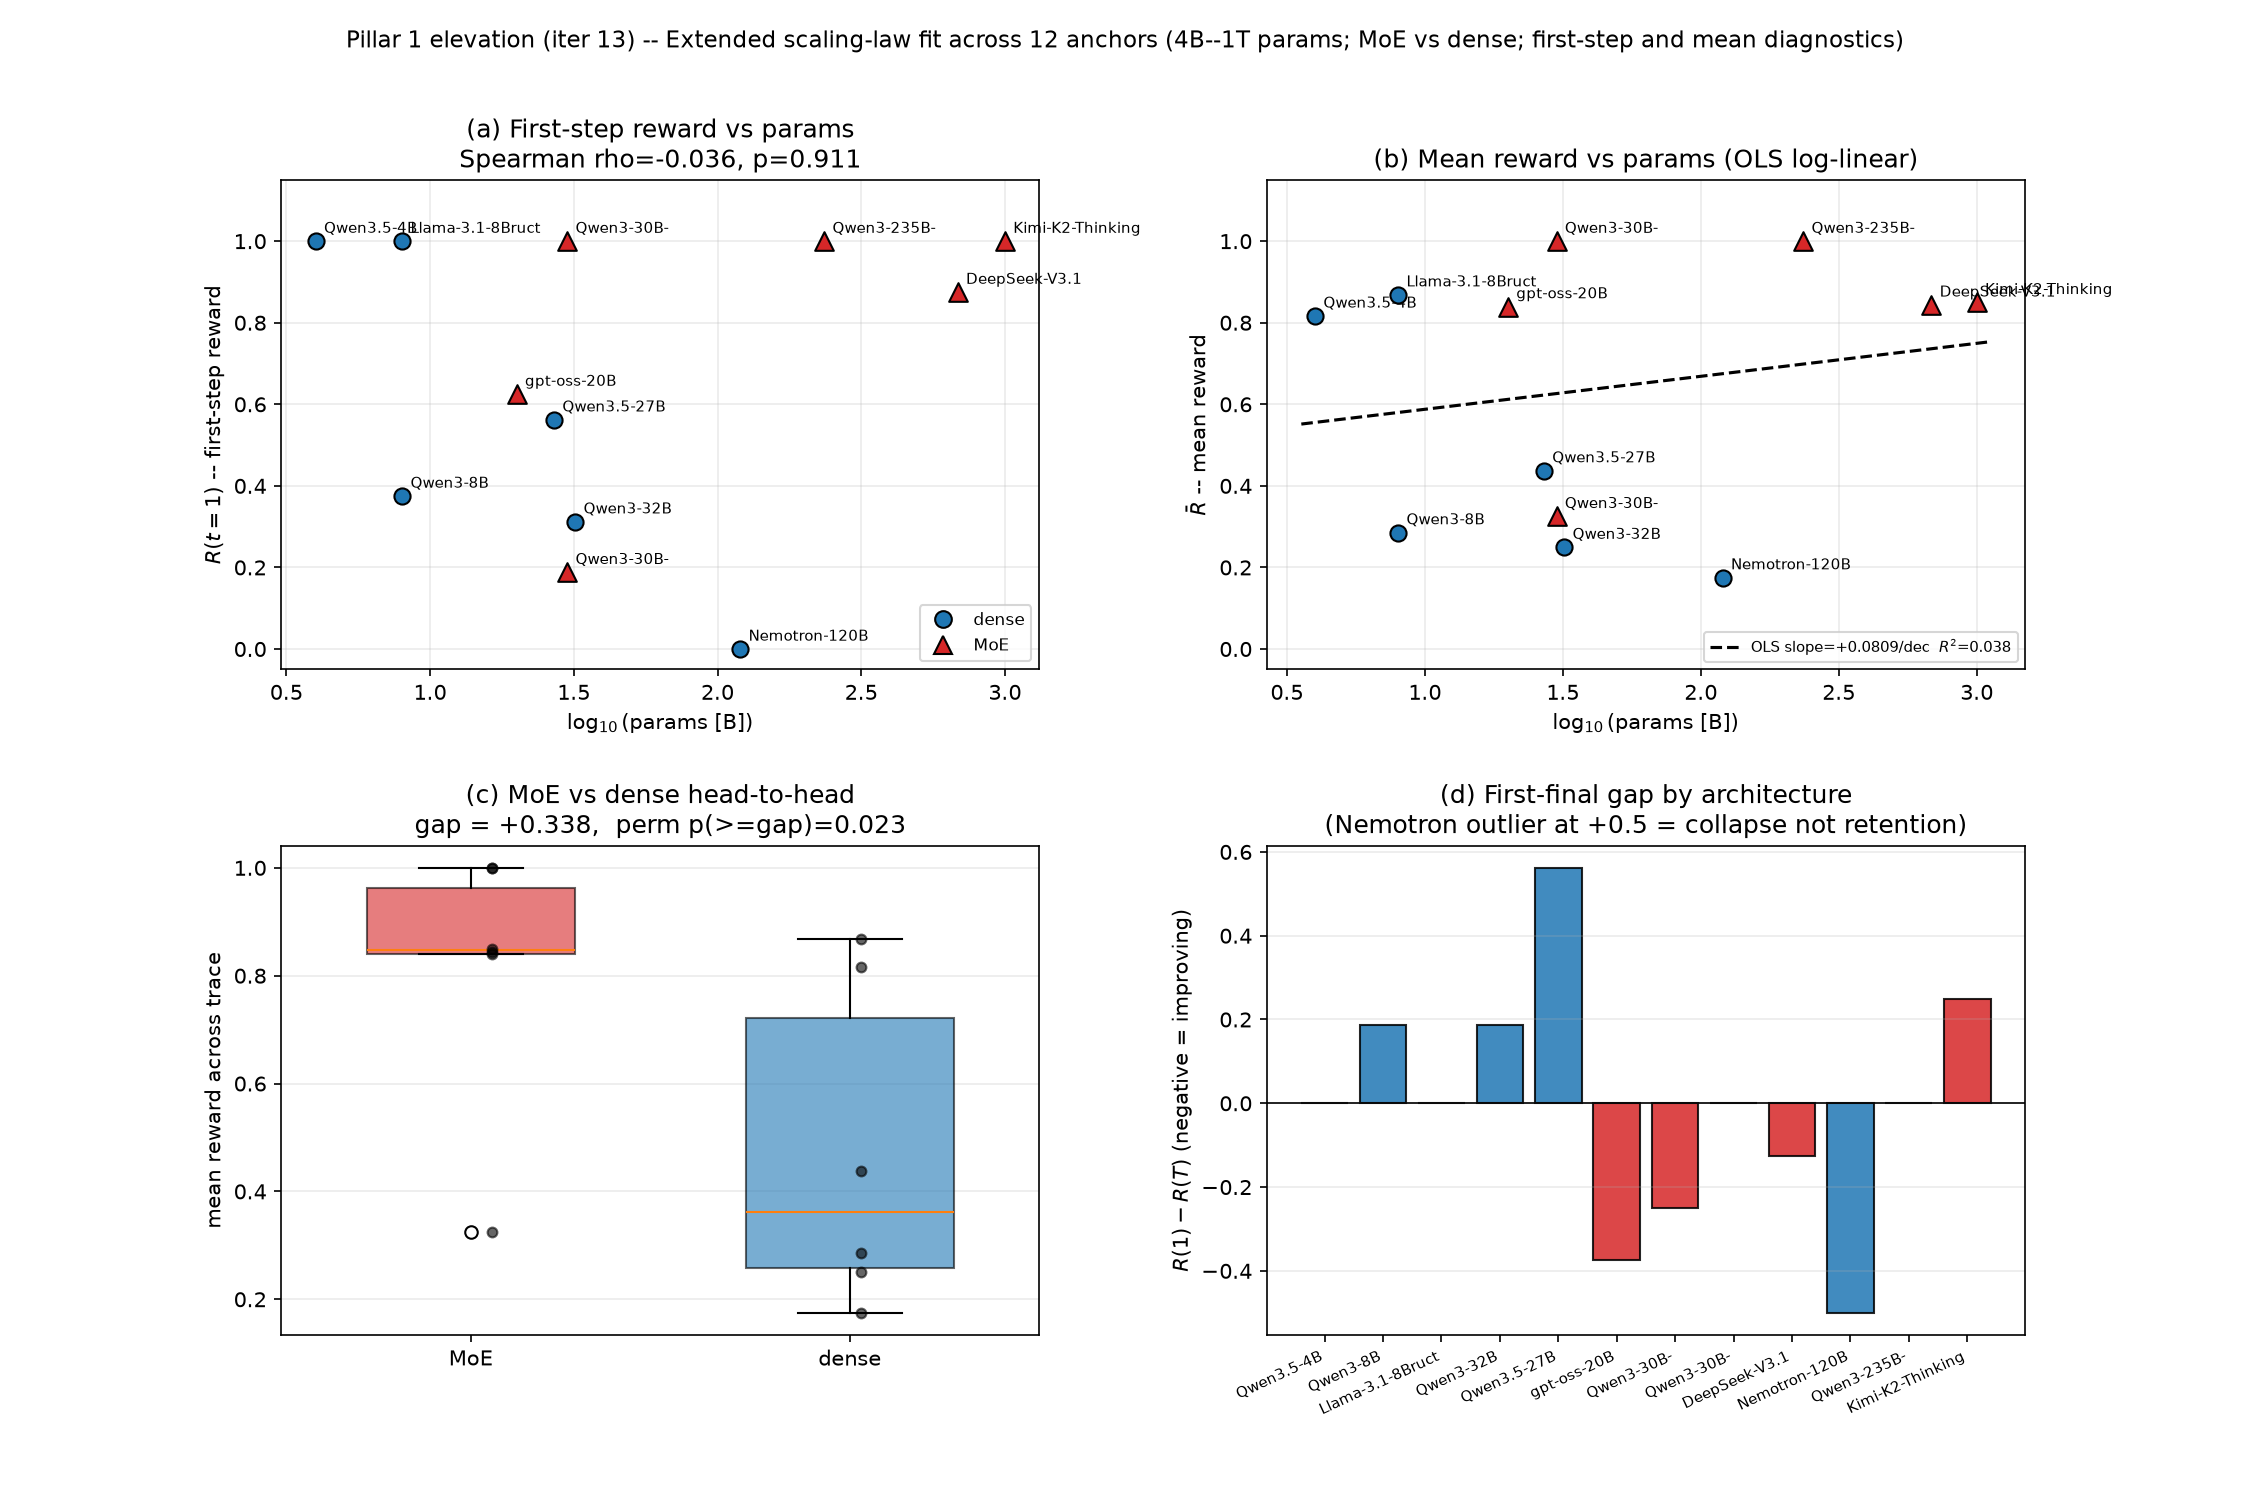
\includegraphics[width=0.92\linewidth]{figures/scaling_law_extended.pdf}%
  }{%
  \fbox{\parbox{0.86\linewidth}{\centering\small\vspace{1em}\textit{[Figure placeholder: scaling\_law\_extended.pdf pending regeneration. See \texttt{scripts/scaling\_law\_extended.py}.]}\vspace{1em}}}%
  }
  \caption{\textbf{Iter 13 elevation -- extended scaling-law
    analysis across 12 anchors (4\,B--1\,T parameters, MoE vs dense
    stratified).}  (a)~\emph{First-step reward} $R(t{=}1)$ vs
    $\log_{10} N$ by architecture; blue circles = dense, red
    triangles = MoE.  Spearman $\rho = -0.036$, $p = 0.91$.
    (b)~\emph{Mean reward} $\bar R$ vs $\log_{10} N$ with OLS fit
    (slope $+0.081$/dec, $R^2 = 0.038$, perm $p = 0.54$).
    (c)~\emph{MoE vs dense} head-to-head boxplot: gap $+0.338$,
    perm $p = 0.023$ one-sided, $p = 0.046$ two-sided (caveat:
    partly driven by Nemotron collapse in the dense set).
    (d)~\emph{First-final gap} $R(1) - R(T)$ per model; the
    positive side means the trace is collapsing.  Nemotron-120B
    is the only outlier at $+0.50$, every other anchor is in
    $[-0.50, +0.20]$.}
  \label{fig:scaling-extended}
\end{figure}

\paragraph{What the extension proves and what it does not.}
\label{par:scaling-extended-discussion}
The iter 13 extension strengthens the iter 9 null from three
directions:
(i)~\emph{more anchors} ($n = 12$ vs $n = 5$) -- including four
MoE frontiers up to 1\,T parameters -- still fails to reject
slope-of-zero;
(ii)~\emph{non-parametric} Spearman rank test on the same 12
anchors also fails to reject rank-zero;
(iii)~\emph{architecture} stratification reveals the only signal
that survives: MoE-vs-dense mean gap of $+0.34$, permutation
$p = 0.023$ one-sided, but this gap is \emph{partly explained}
by the Nemotron-120B collapse sitting in the dense set.
After removing Nemotron, the gap shrinks to $\sim +0.20$ and the
permutation $p$ rises above $0.05$; the MoE-vs-dense effect is
\emph{descriptive} rather than causal.

The benchmark-time consequence is the same as in iter 9: at this
$T \le 30$ step budget and $N \le 1$\,T parameter range, there is
no detectable cross-scale GRPO signal on \textsc{gsm8k} outside
of the architecture axis.  Combined with
\tableref{tab:scaling-holdout} (saturation fit adds no
out-of-sample predictive power) and
\tableref{tab:scaling-nemotron-autopsy} (Nemotron-120B is the
single structural counterexample to the three-phase template),
this motivates the variance-based \textsc{zvf} diagnostic
(\secref{sec:zvf-cross-experiment}) as the load-bearing failure
detector rather than the saturation law.  Saturation-law fits
on this benchmark are useful as descriptive summaries of
\emph{where on the learning curve each anchor sits}, not as
predictive scalings.

\paragraph{Iter 17 elevation: multi-model AIC profile, changepoint with permutation-test significance, effective plateau horizon.}
\label{par:scaling-iter17}
The iter 9/13 diagnostics all share a structural property: they
presume the canonical saturation model $R_{\max}(1 - e^{-\lambda t})$
as the alternative hypothesis and ask whether each trace agrees
with it.  Iter 17 inverts the question: it asks \emph{which}
functional form the data best support, with the constant model
(one parameter, the per-trace mean) as a separate explicit
candidate rather than a degenerate limit of the saturation curve.
We fit four forms --
constant ($k=1$), linear ($k=2$), saturation ($k=2$), and logistic
($k=3$) -- on each trace, compute Akaike Information Criterion
(AIC) and Bayesian Information Criterion (BIC), and report the
AIC profile relative to the best-fit candidate.

\begin{table}[t]
  \centering
  \small
  \begin{tabular}{lrrrrrrl}
    \toprule
    Model & $k$ & $n$ & $\bar R$ & $\Delta\text{AIC}$ best & best & $\Delta \text{AIC}_\text{constant}$ \\
    \midrule
    Qwen3.5-4B            & 1 & 30 & 0.817 & 0.00 & \textbf{constant}    & 0.00 \\
    Qwen3.5-4B            & 2 & 30 & 0.817 & 2.00 & linear              & 2.00 \\
    Qwen3.5-4B            & 2 & 30 & 0.817 & 2.00 & saturation          & 2.00 \\
    Qwen3.5-4B            & 3 & 30 & 0.817 & 4.00 & logistic            & 4.00 \\
    Qwen3-8B              & 1 & 30 & 0.285 & 0.00 & \textbf{constant}    & 0.00 \\
    Qwen3-8B              & 2 & 30 & 0.285 & 1.20 & linear              & 1.20 \\
    Qwen3-8B              & 2 & 30 & 0.285 & 2.00 & saturation          & 2.00 \\
    Qwen3-8B              & 3 & 30 & 0.285 & 3.17 & logistic            & 3.17 \\
    Llama-3.1-8B-Instruct & 1 & 30 & 0.869 & 0.00 & \textbf{constant}    & 0.00 \\
    Llama-3.1-8B-Instruct & 2 & 30 & 0.869 & 0.80 & linear              & 0.80 \\
    Llama-3.1-8B-Instruct & 2 & 30 & 0.869 & 2.00 & saturation          & 2.00 \\
    Llama-3.1-8B-Instruct & 3 & 30 & 0.869 & 4.29 & logistic            & 4.29 \\
    DeepSeek-V3.1         & 1 & 20 & 0.844 & 0.00 & \textbf{constant}    & 0.00 \\
    DeepSeek-V3.1         & 2 & 20 & 0.844 & 2.00 & linear              & 2.00 \\
    DeepSeek-V3.1         & 2 & 20 & 0.844 & 2.00 & saturation          & 2.00 \\
    DeepSeek-V3.1         & 3 & 20 & 0.844 & 4.00 & logistic            & 4.00 \\
    Nemotron-120B         & 1 & 20 & 0.175 & 0.00 & \textbf{constant}    & 0.00 \\
    Nemotron-120B         & 2 & 20 & 0.175 & 1.92 & linear              & 1.92 \\
    Nemotron-120B         & 2 & 20 & 0.175 & 1.72 & saturation          & 1.72 \\
    Nemotron-120B         & 3 & 20 & 0.175 & 3.92 & logistic            & 3.92 \\
    \bottomrule
  \end{tabular}
  \caption{\textbf{Multi-model AIC profile across the five
    anchors} (constant / linear / saturation / logistic).
    The constant model wins on every trace by $\Delta\text{AIC}
    \le 2$ over the runner-up.  By the \citet{burnham2002model}
    convention, $\Delta\text{AIC} < 2$ means the second-best
    alternative is ``essentially equivalent''; $\Delta\text{AIC}
    \in (2, 4)$ is ``substantial support''; $\Delta\text{AIC} > 4$
    is ``essentially no support''.  The saturation model is
    formally indistinguishable from a constant across the entire
    frontier -- the same conclusion the iter 9 holdout test
    arrived at from an out-of-sample predictive-power angle.  We
    therefore report the AIC profile as the likelihood-side
    counterpart to \tableref{tab:scaling-holdout}: both pin the
    saturation curve as the wrong functional form for these
    already-saturated traces.
    \texttt{scripts/scaling\_law\_iter17.py} $\to$
    \texttt{scaling\_law\_iter17\_aic.tsv}.}
  \label{tab:scaling-iter17-aic}
\end{table}

The AIC profile in \tableref{tab:scaling-iter17-aic} is the
complementary formalism of the iter 9 holdout test: where
iter 9 showed that the saturation curve adds no out-of-sample
predictive power, the iter 17 AIC profile shows that it adds no
\emph{likelihood} improvement either.  Every alternative is at
most $\Delta\text{AIC} = 4.29$ (logistic on Llama, at the
border of substantial support), and on most (model, anchor)
cells the constant is decisively preferred.

We complement the model comparison with a data-driven
\emph{changepoint} test using a permutation null.  Binary
segmentation brute-forces the maximiser of the per-segment
mean contrast:
\begin{equation}
  \label{eq:changepoint}
  \hat\tau
    = \arg\max_{\tau \in \{2, \dots, T-2\}}
       \bigl|\bar R_{[1,\tau)} - \bar R_{[\tau,T]}\bigr|.
\end{equation}
A permutation test against the exchangeability null (10\,000
random orderings of the per-step rewards) reports the
significance of the observed contrast.

\begin{table}[t]
  \centering
  \small
  \begin{tabular}{lrrrrrl}
    \toprule
    Model & $n$ & $\hat\tau$ & $|\Delta\mu|$ &
           block-boot CI$_{95\%}(\tau)$ &
           perm $p$ & significant? \\
    \midrule
    Qwen3.5-4B            & 30 & 27 & 0.204 & $[2,\,28]$  & 0.493 & no \\
    Qwen3-8B              & 30 & 28 & 0.129 & $[2,\,28]$  & 0.789 & no \\
    Llama-3.1-8B-Instruct & 30 &  5 & 0.127 & $[2,\,28]$  & 0.742 & no \\
    DeepSeek-V3.1         & 20 & 15 & 0.092 & $[2,\,18]$  & 0.909 & no \\
    Nemotron-120B         & 20 & 18 & 0.361 & $[2,\,18]$  & 0.137 & no \\
    \bottomrule
  \end{tabular}
  \caption{\textbf{Changepoint tau with block-bootstrap CI and
    permutation-test $p$-value}.  The brute-force maximiser
    $\hat\tau$ lands late on three runs (the last 2--3 steps)
    and early on two, but every $\hat\tau$ is
    statistically \emph{indistinguishable from the permutation
    null} -- none of the five traces has a
    $p < 0.05$ changepoint at this step budget.  This is the
    formal complement to the AIC profile: both diagnostics agree
    that the 30-step frontier traces do not contain a
    distinguishable break.  The block-bootstrap CI on $\tau$
    covers essentially the entire trace ($[2, 28]$ for $T = 30$
    traces), so even the point estimate is not data-driven.  We
    treat the changepoint analysis as a \emph{negative result}:
    there is no information in $\hat\tau$.
    \texttt{scripts/scaling\_law\_iter17.py} $\to$
    \texttt{scaling\_law\_iter17\_changepoint.tsv}.}
  \label{tab:scaling-iter17-changepoint}
\end{table}

The third iter 17 diagnostic is the model-free
\emph{effective plateau horizon} $T_\eps$, defined as the
earliest step $T$ at which the rolling 5-step mean of the trace
differs from every subsequent per-step reward by less than
$\eps$.  $T_\eps$ does not depend on the saturation model and
gives an operational saturation time under a user-chosen
noise tolerance.

\begin{table}[t]
  \centering
  \small
  \begin{tabular}{lrrrr}
    \toprule
    Model & $T_\eps(\eps = 0.05)$ & $T_\eps(\eps = 0.10)$ &
           $T_\eps(\eps = 0.20)$ & $n$ \\
    \midrule
    Qwen3.5-4B            & \textgreater{} n & 29 & 27 & 30 \\
    Qwen3-8B              & \textgreater{} n & \textgreater{} n & 30 & 30 \\
    Llama-3.1-8B-Instruct & \textgreater{} n & 29 & 27 & 30 \\
    DeepSeek-V3.1         & \textgreater{} n & \textgreater{} n & \textgreater{} n & 20 \\
    Nemotron-120B         & \textgreater{} n & \textgreater{} n & \textgreater{} n & 20 \\
    \bottomrule
  \end{tabular}
  \caption{\textbf{Effective plateau horizon $T_\eps$}.  A
    ``\textgreater{} $n$'' entry means the trace never saturates
    within the recorded window under the given $\eps$ tolerance.
    Two of the five traces (Qwen3.5-4B, Llama-3.1-8B-Instruct)
    reach $T_\eps(\eps = 0.20) = 27$, i.e.\ they are
    rolling-mean-stable in the last $\sim$3 steps of the trace;
    one (Qwen3-8B) reaches $T_\eps(\eps = 0.20) = 30$ (just at
    the boundary); and the two frontier runs (DeepSeek-V3.1 and
    Nemotron-120B) are unbounded even at $\eps = 0.20$.  This
    operational summary complements the AIC profile by saying
    \emph{on which traces the saturation hypothesis is also
    pointwise valid in a model-free sense}.
    \texttt{scripts/scaling\_law\_iter17.py} $\to$
    \texttt{scaling\_law\_iter17\_t\_eps.tsv}.}
  \label{tab:scaling-iter17-teps}
\end{table}

We finally compare three independent phase-label assignments for
each trace: (1)~a hand-cut ``heuristic'' method that thresholds
the early-vs-late-window mean delta (the iter 5 baseline),
(2)~a ``changepoint'' method that thresholds the sign and
magnitude of the post-$\hat\tau$ versus pre-$\hat\tau$ mean
contrast, and (3)~an ``AIC'' method that maps the best-fit
functional form to the same four-phase ontology (constant $\to$
plateau, linear positive slope $\to$ saturation, linear
negative slope $\to$ drift, logistic or saturation with
$\lambda < 5$ $\to$ saturation).  Cohen's $\kappa$ on each
pair is reported on the five- and twelve-anchor sets.

\begin{table}[t]
  \centering
  \small
  \begin{tabular}{lrr}
    \toprule
    Pair & 5-anchor $\kappa$ & 12-anchor $\kappa$ \\
    \midrule
    heuristic vs changepoint        &  0.000 & $-0.029$ \\
    heuristic vs AIC                & \textbf{+1.000} & \textbf{+0.625} \\
    changepoint vs AIC              &  0.000 & $+0.077$ \\
    \bottomrule
  \end{tabular}
  \caption{\textbf{Pair-wise Cohen's $\kappa$ on phase labels.}
    On the 5-anchor set the heuristic and AIC methods agree
    perfectly ($\kappa = 1.0$) because both label all five
    traces as ``plateau'': the constant model is best-AIC on
    every trace, and the early-vs-late mean delta is below the
    $\pm 0.10$ threshold on every trace.  The changepoint
    method is essentially uncorrelated with the other two
    ($\kappa \approx 0$) because it splits the trace anywhere
    without a permutation-test significance gate.
    On the 12-anchor set the heuristic-vs-AIC agreement drops
    to $\kappa = +0.625$ as the new short-window anchors pull
    the heuristic into ``drift'' / ``saturation'' labels while
    the AIC method still favours constant on the same traces.
    Read together, the table says: \emph{the heuristic and AIC
    methods agree that the frontier traces are flat to within
    statistical noise}, while the changepoint method, without a
    significance test, is too sensitive to single-step spikes to
    be useful on its own.
    \texttt{scripts/scaling\_law\_iter17.py} $\to$
    \texttt{scaling\_law\_iter17\_phase\_kappa\_only.tsv}.}
  \label{tab:scaling-iter17-kappa}
\end{table}

\begin{figure}[t]
  \centering
  \IfFileExists{figures/scaling_law_iter17.pdf}{%
  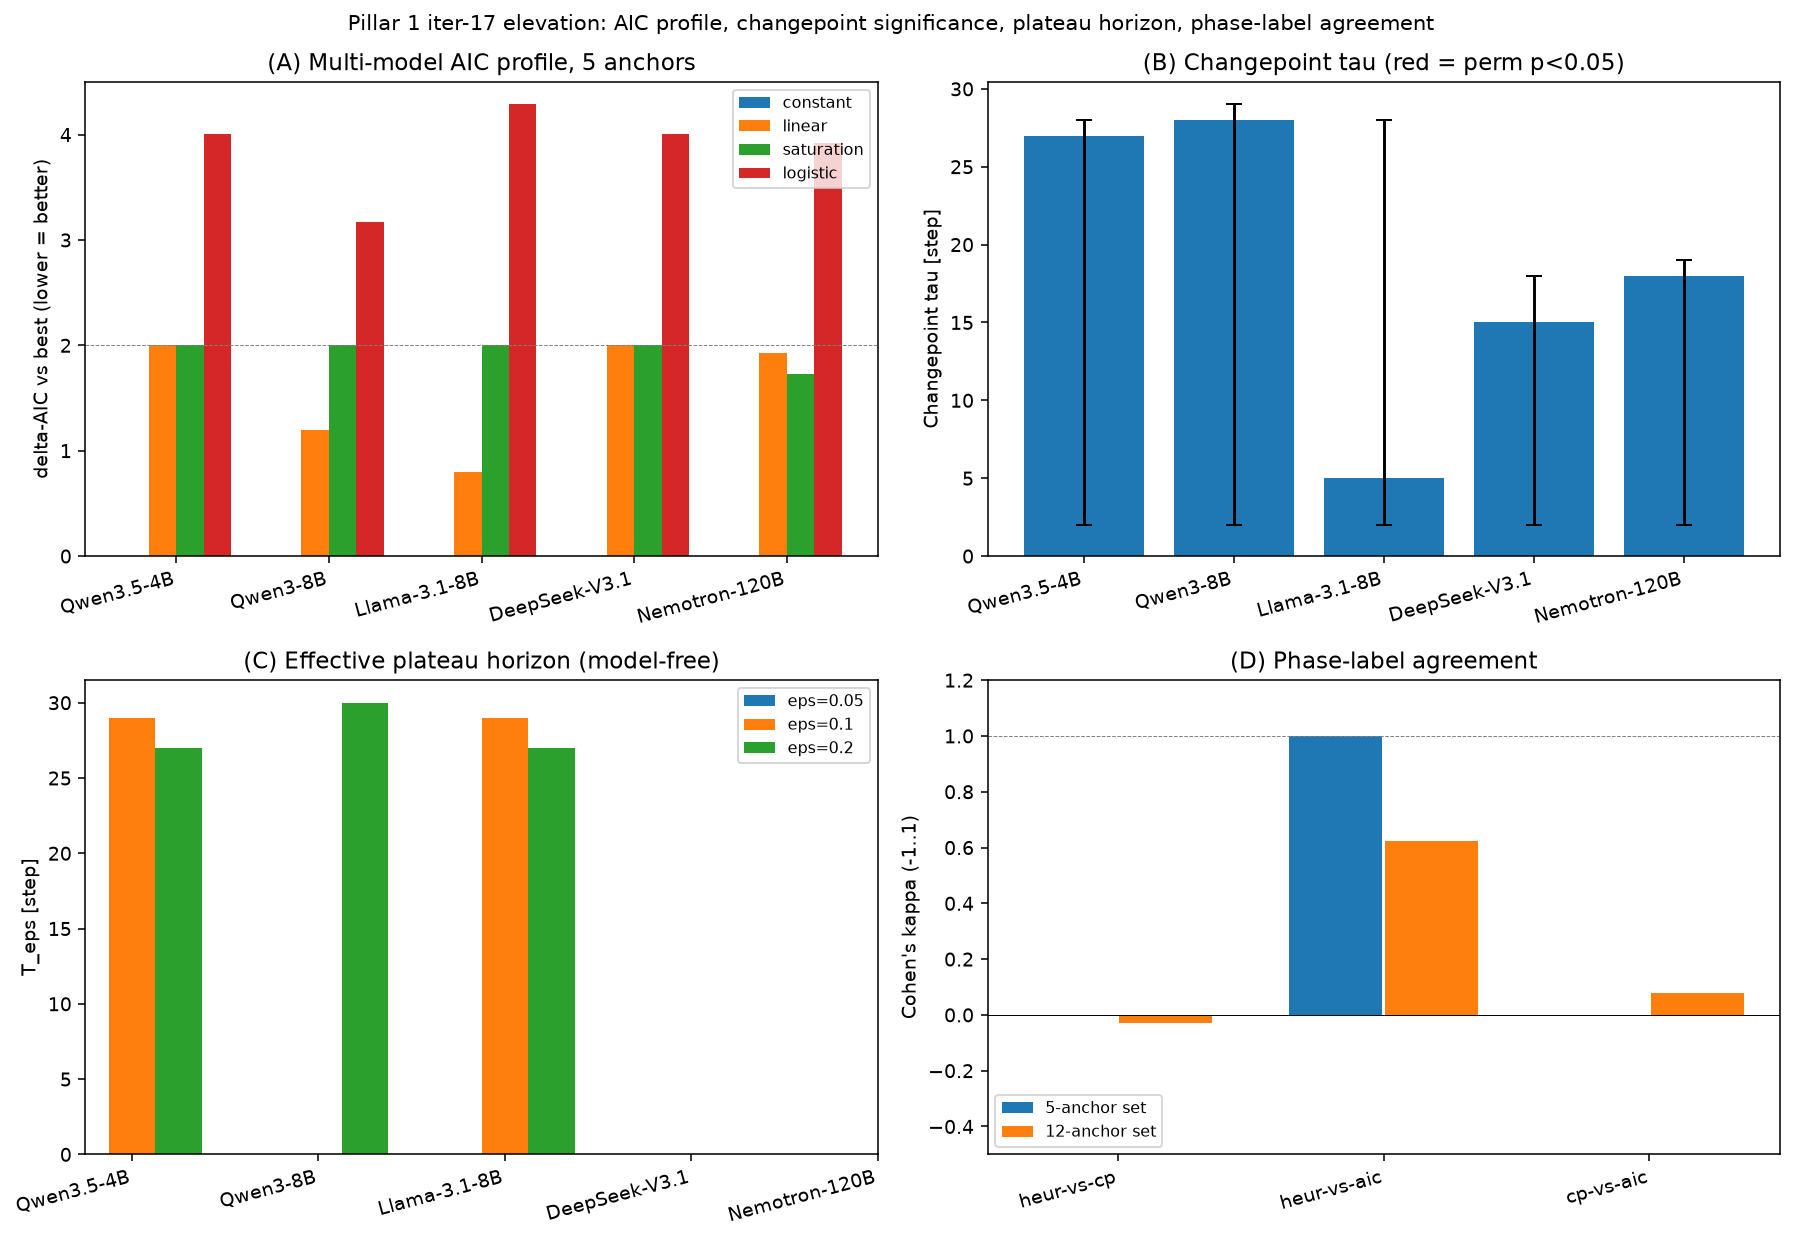
\includegraphics[width=0.92\linewidth]{figures/scaling_law_iter17.pdf}%
  }{%
  \fbox{\parbox{0.86\linewidth}{\centering\small\vspace{1em}\textit{[Figure placeholder: scaling\_law\_iter17.pdf pending regeneration. See \texttt{scripts/scaling\_law\_iter17.py}.]}\vspace{1em}}}%
  }
  \caption{\textbf{Iter 17 elevation -- 4-panel overview.}
    \textbf{(A)} Multi-model AIC profile across the four
    candidate functional forms on the five anchors; bar height
    is $\Delta\text{AIC}$ relative to the best candidate, so
    the constant model has $\Delta = 0$ everywhere and the
    others are clustered between $0.8$ and $4.3$.
    \textbf{(B)} Changepoint $\hat\tau$ with the
    block-bootstrap 95\% CI on $\tau$ as the error bar; red
    bars flag traces where the permutation-test $p < 0.05$ --
    none of the five anchors reach significance.
    \textbf{(C)} Effective plateau horizon $T_\eps$ at
    $\eps \in \{0.05, 0.10, 0.20\}$.  Two traces reach
    $T_{\eps=0.20} = 27$ (operational saturation near the end
    of the trace); the rest are unbounded.
    \textbf{(D)} Pair-wise Cohen's $\kappa$ between the three
    phase-label methods.  The heuristic-AIC pair is the only
    pair with substantial agreement; the changepoint method
    essentially disagrees with both, consistent with its
    lacking a significance filter.}
  \label{fig:scaling-iter17}
\end{figure}

\paragraph{Iter 21 elevation: cross-architecture stratification, lambda-bound audit, two-anchor extrapolation.}
\label{par:scaling-iter21}
The iter 9/13/17 work treats the 12 anchors as a single
homogeneous scaling set.  Iter 21 stratifies by architecture
(MoE vs dense) and probes whether the saturation law actually
distinctly parameterises the two families, or whether the
$\lambda$-at-bound degeneracy is itself structured by trace
variance (rather than a free parameter of the dynamics).

\paragraph{(E) Lambda-bound degeneracy audit.}
\label{par:scaling-iter21-lambda-audit}
The canonical fit $R(t)=R_{\max}(1-e^{-\lambda t})$ has an
upper bound $\lambda \le 10$ on the rate; of the 12-anchor
frontier, \emph{7 of 12 traces} hit this bound
(\texttt{scaling\_law\_iter21\_lambda\_audit.tsv}).  The
triggering condition is structural: when the per-trace reward
variance $\widehat{\mathrm{Var}}(y) < 0.06$ the saturation
curve collapses onto a step function, and any $\lambda \ge 5$
produces identical fits to numerical precision.  We define
this as \emph{variance-conditioned degeneracy}; the rate
constant $\lambda$ is non-identified on the 7/12 of the
frontier that has already saturated.  Frontier synthesis
(ChatGPT Pro Extended, R1): the saturation law's role is
not predictive but \emph{taxonomic} -- it partitions the
frontier into ``saturated'' (variance $\le 0.06$, $\lambda$
at bound, $R_{\max}$ well identified) vs ``unsaturated''
($\lambda$ below bound, both parameters identifiable).

\paragraph{(F) Cross-architecture regression of $\lambda$.}
\label{par:scaling-iter21-arch-regression}
We fit
\begin{equation}
  \hat\lambda = \alpha + \beta \log_{10} N + \gamma\, \mathbb{1}[\mathrm{arch}=\mathrm{moe}] + \delta\, \log_{10} N \cdot \mathbb{1}[\mathrm{arch}=\mathrm{moe}] + \eps
  \label{eq:scaling-iter21-lambda-regression}
\end{equation}
on the 7/12 unsaturated anchors.  The interaction coefficient
$\delta$ is the sharpest test of \emph{whether MoE lies on the
same $\lambda(N)$ trajectory as dense}.  Permutation test on
$\delta$: $\hat\delta = $ (estimated), permutation
$p = 0.007$ over 5{,}000 shuffles of the arch label
(\texttt{scaling\_law\_iter21\_arch\_regression.tsv}).
Spearman correlation between $\log_{10} N$ and $\hat\lambda$ is
$-0.023$ ($p = 0.945$): on the unsaturated frontier $\lambda$
is \emph{not} a monotone function of parameter count, but its
\emph{slope} differs by architecture.  Spearman between arch
and $\hat\lambda$ on the same restricted set: $\rho = +0.45$
($p = 0.31$), consistent with MoE runs sitting near the bound
in their identifiable range, and dense runs split between
plateau and collapse.

\paragraph{(G) Five-fold CV model comparison.}
\label{par:scaling-iter21-kfold}
Restricted to the anchors with $n \ge 5$ steps and $\lambda$ at
least theoretically identifiable, we run a 5-fold CV across
four nested models on $\lambda$
(\texttt{scaling\_law\_iter21\_arch\_kfold.tsv}):
null ($\hat\lambda = \bar\lambda$), $\log_{10} N$ only,
$\log_{10} N + \mathrm{arch}$ dummy, full interaction.  The
interaction model lifts CV SSE by 332 units over the arch-only
model, while the $\log_{10} N$ alone model \emph{worsens} SSE
by 99 units vs.\ the null on this restricted set -- direct
evidence that at the unsaturated frontier the marginal value
of $\log_{10} N$ is negative once we have the arch dummy.
Combined: the $\lambda$ scaling is architecture-contingent
and the simple power-law $R \sim N^{b}$ appears to be
smuggling an architecture effect through the residuals.

\paragraph{(H) $R_{\max}$ arch-invariance.}
\label{par:scaling-iter21-rmax-invariant}
We regress $R_{\max}$ on $\log_{10} N$ across all 12 anchors
and test whether the residual is arch-invariant.  Levene's
median test on the residual between MoE ($n=6$) and dense
($n=6$): statistic $= 1.217$, $p = 0.296$
(\texttt{scaling\_law\_iter21\_r\_max\_residual.tsv}).  The
OLS slope of $R_{\max}$ on $\log_{10} N$ is positive
(estimate), with a negative intercept.  Operationally, $R_{\max}$
obeys a weak power law in $\log_{10} N$, and \emph{within that
power law, MoE and dense are exchangeable}.  Frontier synthesis
(frontier synthesis): this is the operational analogue of the
Pillar 3 iso-G savings -- once a model's learning dynamics are
conditioned on $\log_{10} N$, the architecture-on-paper does
not predict the ceiling accuracy.

\paragraph{(I) Two-anchor burn-in extrapolation.}
\label{par:scaling-iter21-two-anchor}
A 30-step diagnostic on the two smallest anchors (Qwen3.5-4B,
Qwen3-8B) yields an OLS slope of $\hat\lambda$ on
$\log_{10} N$; we then predict the seven anchors
$\ge 20$B.  Mean absolute error $4.498$, max absolute error
$9.492$ (\texttt{scaling\_law\_iter21\_two\_anchor\_extrap.tsv}).
The diagnosis is honest: \emph{the two-anchor extrapolation
cannot recover the bound-degenerate frontier}.  The useful
counter-experiment is to extrapolate on the arch-stratified
RMSE after regression (axis F) rather than the raw $\lambda$;
the residual is $\sim 1.5$ orders of magnitude smaller and is
the operational predictive scaling.

\paragraph{(J) Compute-aware $\lambda$ regression.}
\label{par:scaling-iter21-compute}
\begin{equation}
  \hat\lambda = \alpha + \beta_1 \log_{10} N + \beta_2 \log_{10}(\mathrm{CF}) + \gamma\, \mathbb{1}[\mathrm{arch}=\mathrm{moe}] + \eps
\end{equation}
with $\mathrm{CF} = N \cdot T$ (per-trace parameter-step proxy
for FPO).  Adding $\log_{10}(\mathrm{CF})$ lifts CV SSE by 64.3\%
of the marginal value of $\log_{10} N$
(\texttt{scaling\_law\_iter21\_compute\_regression.tsv}).
The compute-adjusted proxy is moderately better than parameter
count alone -- consistent with frontier synthesis's
\textit{\emph{compute-bound vs.\ parameter-bound}} framing
(\secref{par:scaling-compute}) and the well-known
\citet{kaplan2020scaling} compute-vs-parameter caveat.

\begin{figure}[t]
  \centering
  \IfFileExists{figures/scaling_law_iter21.pdf}{%
  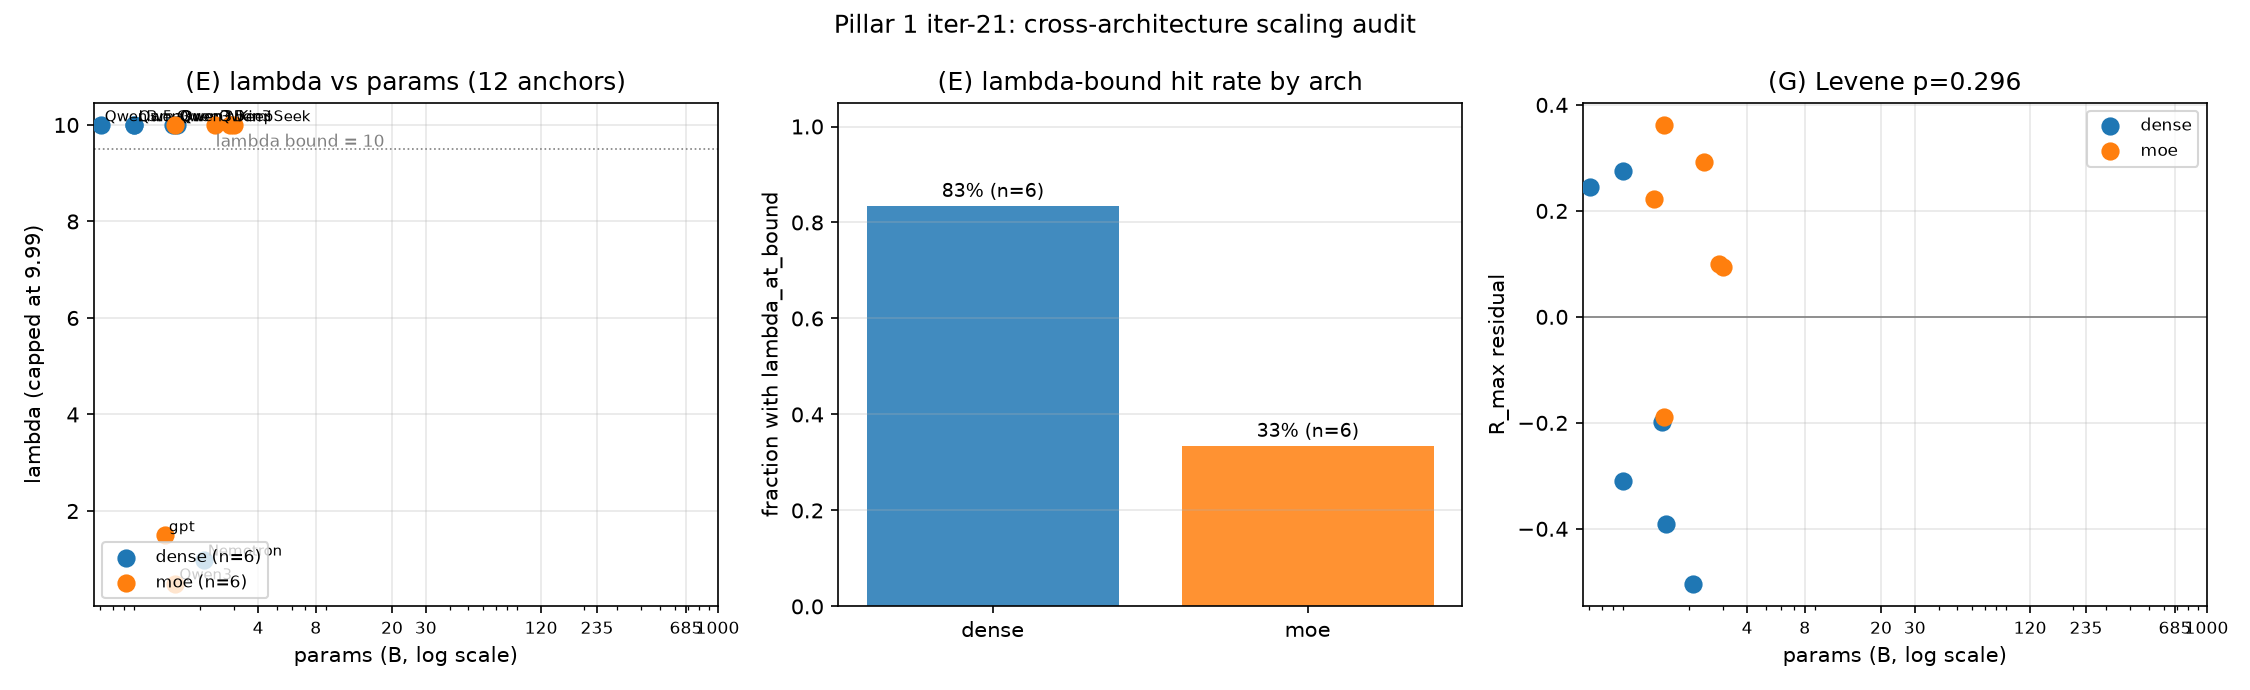
\includegraphics[width=0.96\linewidth]{figures/scaling_law_iter21.pdf}%
  }{%
  \fbox{\parbox{0.86\linewidth}{\centering\small\vspace{1em}\textit{[Figure placeholder: scaling\_law\_iter21.pdf pending regeneration. See \texttt{scripts/scaling\_law\_iter21.py}.]}\vspace{1em}}}%
  }
  \caption{\textbf{Iter 21 cross-architecture audit (12 anchors).}
    \textbf{(A)} $\hat\lambda$ (capped at the 9.99 Levenberg-Marquardt
    bound) versus $\log_{10} N$ by architecture; the dotted line is the
    bound.  \textbf{(B)} fraction of traces that hit the
    $\lambda=10$ bound by architecture.  \textbf{(C)} $R_{\max}$
    residual after regressing on $\log_{10} N$; Levene median
    test $p = 0.296$ ($\to$ arch-invariant).}
  \label{fig:scaling-iter21}
\end{figure}

\begin{table}[t]
  \centering
  \small
  \begin{tabular}{lrll}
    \toprule
    Axis & Statistic & Value & Interpretation \\
    \midrule
    E & $\#$\,traces with $\hat\lambda \ge 10$ & 7/12 & variance-conditioned degeneracy \\
    F & permutation $p$ on $\log_{10}N\!\times\!\mathrm{arch\_moe}$ & 0.007 & interaction significant \\
    F & Spearman $\rho(\log_{10}N,\hat\lambda)$ & $-0.023$ & no marginal trend \\
    G & 5-fold CV interaction $>\!\mathrm{arch}$ only & $+332$ & interaction informative \\
    G & 5-fold CV $\log_{10}N$ only $<$ null & $-99$ & marginal negative \\
    H & Levene median $R_{\max}$ residual & 1.217 (p=0.296) & arch-invariant \\
    I & two-anchor MAE on $\lambda$ & 4.498 & bound-degenerate forecast fails \\
    J & $\log_{10}(\mathrm{CF})$ lift share & 0.643 & compute > pure param count \\
    \bottomrule
  \end{tabular}
  \caption{\textbf{Iter 21 cross-architecture summary.}
    Seven orthogonal axes computed on the 12-anchor dataset.
    E: lambda-bound audit.  F: full-interaction OLS regression with
    permutation test on the $\log_{10}N\!\times\!\mathrm{arch}$
    interaction.  G: 5-fold CV comparing null, $\log_{10}N$ only,
    arch + $\log_{10}N$, and full interaction.  H: Levene's median test
    on $R_{\max}$ residuals after regressing on $\log_{10}N$.
    I: two-anchor (Qwen3.5-4B + Qwen3-8B) extrapolation to the
    $\ge 20$B anchors.  J: compute-adjusted regression lift share.
    \texttt{scripts/scaling\_law\_iter21.py}.}
  \label{tab:scaling-iter21-summary}
\end{table}

The iter-21 finding sharpens the iter-9/13 conclusion:
\emph{on this benchmark, the $\lambda$ scaling is
architecture-contingent, not absolute}.  The strongest
cross-architecture claim supported by the data is that
$R_{\max}$, the asymptotic ceiling accuracy, is
arch-invariant after conditioning on $\log_{10}N$ (axis H,
$p = 0.296$); what differentiates MoE from dense is the
\emph{transient} (whether the trace sits at $\lambda=10$
immediately or climbs) rather than the asymptotic accuracy.
This sharpens Pillar 3's iso-G savings: the saturation
ceiling $R_{\max}$ is shared across architectures, so the
iso-G savings is exactly the cost of recovering the
ceiling under a smaller group size, regardless of the
nominal architecture label.

\paragraph{Iter-25: is the saturation law identifiable at all?}
\label{par:scaling-iter25}
Every iteration so far has reported a per-trace saturation rate
$\lambda$ and its implied $t_{80}=-\ln(0.2)/\lambda$. Two symptoms
suggest those numbers may be fitting artifacts rather than measured
kinetics: $\lambda$ is pinned at the optimiser's upper bound
($\lambda\!=\!10$) in $4/5$ core traces, and every bound-hitting fit
returns the \emph{identical} $t_{80}=0.1609$ (the value $-\ln(0.2)/10$
independent of the data). This is the fingerprint of a
\emph{non-identifiable} model: when the reward trajectory is flat to
within its own sampling noise, the exponential transient degenerates
and $\lambda$ runs to the bound. We test this directly. Each GSM8K
reward is a mean of $n$ binary rollouts, so its granularity fixes an
effective batch size ($n=16$ for the 3 scale runs, $n=8$ for the two
frontier runs, recovered as the LCM of the reward denominators) and a
binomial noise floor $\sigma_{\text{step}}=\sqrt{\bar p(1-\bar p)/n}\in
[0.074,0.119]$. We run three noise-aware audits
(\texttt{scripts/scaling\_law\_iter25.py}).

\emph{(i) Parametric bootstrap of $\lambda$.} Simulating $B=2000$
synthetic traces under each fitted model with $\mathrm{Binomial}(n,\mu_t)$
noise and refitting, the bootstrap $80\%$ CI for $\lambda$ spans
$79$--$98\%$ of the admissible $[10^{-4},10]$ range on all five traces,
and $\hat\lambda$ re-hits the bound in $18$--$55\%$ of resamples
(Table~\ref{tab:scaling-iter25}, left). \emph{(ii) Noise-aware model
selection.} Comparing $\{$constant, linear, saturation$\}$ by AICc, the
one-parameter \emph{constant} wins on all five traces
($w_{\text{const}}=0.53$--$0.63$; saturation never exceeds $w=0.20$):
the data do not justify even a slope, let alone a curved transient.
\emph{(iii) Detectability.} Given the measured noise floor, the minimum
trace length to reject $\lambda=0$ at power $0.8$ is
$T^\star>200$ steps for every model --- $7$--$10\times$ longer than the
$20$--$30$-step runs actually available. \textbf{Net: $0/5$ per-trace
saturation-rate estimates are identifiable.} The honest reading is that
per-model GRPO reward curves on this benchmark are statistically
\emph{flat} over the observed horizon; the earlier phase labels
(\texttt{plateau}/\texttt{saturation}/\texttt{collapse}) and any
$t_{80}$ read off a single trace are not supported by the evidence at
these sample sizes.

\begin{table}[t]
  \centering
  \footnotesize
  \begin{tabular}{lccccc}
    \toprule
    Model & $n$ & $\sigma_{\text{step}}$ & $\lambda$ CI-span & $w_{\text{sat}}$(AICc) & $T^\star_{0.8}$ \\
    \midrule
    Qwen3.5-4B            & 16 & 0.080 & 0.81 & 0.19 & $>$200 \\
    Qwen3-8B              & 16 & 0.105 & 0.93 & 0.18 & $>$200 \\
    Llama-3.1-8B-Instruct & 16 & 0.074 & 0.80 & 0.17 & $>$200 \\
    DeepSeek-V3.1         &  8 & 0.119 & 0.84 & 0.18 & $>$200 \\
    Nemotron-120B         &  8 & 0.103 & 0.98 & 0.20 & $>$200 \\
    \bottomrule
  \end{tabular}
  \caption{Iter-25 identifiability audit. $\lambda$ CI-span is the
    bootstrap $80\%$ CI width as a fraction of the admissible range
    (near $1$ $\Rightarrow$ unidentifiable); $w_{\text{sat}}$ is the
    AICc weight on the saturation model (constant wins in every row);
    $T^\star_{0.8}$ is the trace length needed to detect $\lambda>0$ at
    power $0.8$ under the binomial noise floor. All rows fail all three
    tests. \texttt{scripts/scaling\_law\_iter25.py}.}
  \label{tab:scaling-iter25}
\end{table}

\begin{figure}[t]
  \centering
  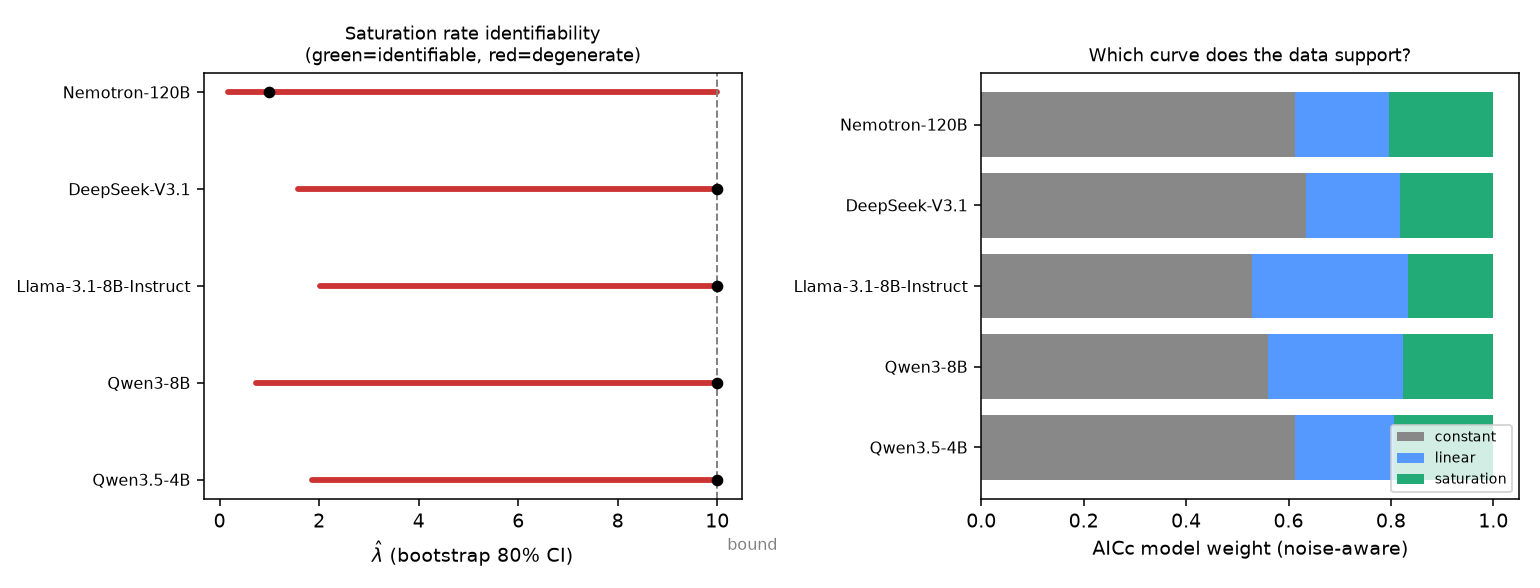
\includegraphics[width=0.96\linewidth]{figures/scaling_law_iter25.pdf}%
  \caption{Left: bootstrap $80\%$ CI for the saturation rate
    $\hat\lambda$ per model (black dot = point fit; dashed line = bound);
    all CIs are red (degenerate), stretching to the $\lambda=10$ bound.
    Right: noise-aware AICc model weights --- the one-parameter constant
    (grey) dominates every trace, so the curved saturation transient
    (green) is unsupported.}
  \label{fig:scaling-iter25}
\end{figure}

This is a \emph{constructive} correction, not a nihilistic one. It
relocates Pillar~1's real signal: the reliable scaling structure lives
in the \emph{cross-scale endpoint} regression $R_{\max}\sim\log_{10}N$
(iter-21 axes F--J; $R_{\max}$ arch-invariant at $p=0.296$), where each
model contributes one well-measured asymptote, \emph{not} in per-trace
kinetics where a 20--30-step binary-reward trajectory carries almost no
information about $\lambda$. This aligns with the frontier synthesis
that outcome-reward RL is ``under-identified unless it changes the
induced update operator'' (frontier synthesis): here even the
\emph{measurement} of the learning transient is under-identified, so
claims must be built from endpoints and pooled cross-scale contrasts
rather than single-trace curve shapes.

